%%
%% CalciumSignalling.tex
%% Login : <hoang-trong@hoang-trong-laptop>
%% Started on  Thu Jun  4 18:05:13 2009 Hoang-Trong Minh Tuan
%% $Id$
%% 
%% Copyright (C) 2009 Hoang-Trong Minh Tuan
%%


\chapter{Calcium Signalling}
\label{chap:calcium-signalling}


\def\IPthreeR{{\text{IP}_3\text{R}}}

The previous chapters have discussed important transmembrane proteins
which act as ionic selectivity pores. Among those ions, \ce{Ca^2+} is
properly the most ubiquitous and most diverse functions. \ce{Ca^2+}
servers as a second messenger for which we will focus in this
Chapter. We will limit our discuss in cardiac myocytes.  Reminding
that in cardiac myocytes, the dominant calcium ion channels is L-type
(aka $\alpha_{1C}$ or $\ce{Ca}_v1.2$ or dihydropyridine receptor
(DHPR)).

\section{Calcium function}
\label{sec:calcium-function}

The role of calcium has been discovered since 1882 by Ringer in his series of
papers (Sect.\ref{sec:Ringer-solution}). 

\begin{enumerate}
  \item excitation - Sect.\ref{sec:cardiac-cycle}
  
  \item insertion of receptors into the membrane - Sect.\ref{sec:Trk}
  
  \item cAMP - Sect.\ref{sec:cAMP}
  
  \item production of IP3 - Sect.\ref{sec:IP3_synthesis}
  
  \item activation of PKC - Sect.\ref{sec:PKC}
  
  \item release neurotransmitters - Sect.\ref{sec:neurotransmitter-release}.
  
\end{enumerate}

\section{What can modulate cytosolic and SR Ca2+ ?}

\begin{enumerate}
  \item ER-membrane channels: IP3R; RyR

NOTE: ER-PM junction (Sect.\ref{sec:junction-ER-plasmamembrane})
  
  \item TNF - Sect.\ref{sec:TNF-alpha}
  
  \item  
\end{enumerate}

\section{Calcium dynamics}
\label{sec:calcium-dynamics}
\label{sec:calcium-homeostasis}


Calcium level in extracellular media, cytosol and ER region:
\begin{itemize}
  \item  1.5 mM, 50 nM, and 400 $\mu$M, respectively in many cell types
  
  \item  1.8 mM, 100 nM, and 1000 $\mu$M, respectively in cardiac myocytes
  
\end{itemize}


As calcium is the second messenger, its change in concentration lead to several
changes in cellular states. By changing the intracellular calcium concentration,
the influx or efflux of \ce{Ca^2+} across cell membranes triggers
(activate/inactivate) many cellular events/processes
(Sect.\ref{sec:calcium-function}).

Under action potential, the cytoplasmic calcium concentration can
increase 10-100 fold, at local regions. Calcium elevation
regulates many cellular events.  The free \ce{Ca^2+} will diffuse to different
compartments in the cell to perform its function by binding to different
molecules. However, the excessive amount of calcium
can cause severe conditions to the cell. 

\subsection{At rest}

In resting condition, calcium concentration is kept at a steady level
with high gradient between extracellular and cytosolic environment.
Due to this low intracellular calcium concentration and high gradient, cells
need many ``tools'' and much energies to keep this low concentration.
The mechanisms that cell controls the $[\ce{Ca^2+}]_i$ is the central interest
in cell physiology.  There are a number of \ce{Ca^2+} control mechanisms
operating on different levels. We will focus on how cell regulating the activity
of these gates.


\begin{framed}
  The concentration of $[\ce{Ca^2+}]_i$ is regulated by `on' reaction
  that introduce (free) \ce{Ca^2+} into the cytoplasm and `off' reaction
  that remove \ce{Ca^2+} by the combined action of buffers, pumps and
  exchangers (Na/Ca exchanger (NCX) and plasma membrane \ce{Ca^2+}
  ATPase (PMCA)) depending upon cell's
  demands\footnote{\url{http://en.wikipedia.org/wiki/Plasma_membrane_Ca2+_ATPase}},
  as shown in Fig.~\ref{fig:Ca_signalling}~\citep{berridge2003csd}. Any
  alteration to this \ce{Ca^2+}-dependent homeostatic mechanism can lead
  to many prominent diseases.  By \ce{Ca^2+} homeostasis, we means that
  \ce{Ca^2+} influxes during the ``off'' reaction exactly match those
  during the ``on'' reaction.

\end{framed}

\subsection{Calcium elevation}

{\bf ``On'' reaction}: stimuli induces the low-level entry of extracellular
\ce{Ca^2+} and the formation of intracellular second messengers (\ce{Ca^2+},
IP3, ADP). E.g. \ce{Ca^2+} and IP3 induce the release of \ce{Ca^2+} stored in
the ER, and its myocyte equivalent, SR. Most of these free ions (shown in red
circles) rapidly bound to the buffers, while some of them bound to the effectors
to activate various cellular processes, e.g. excitation-contraction in
myocardial cells.

% \ce{Ca^2+} enters the myocytes via the L-type calcium channels (LCC)
% and released from the internal calcium storage (SR) via RyR (as
% described in the two previous sections). 
Calcium in the cytosol can come from (with (A) and (B) are the two principal
pathways)
\begin{enumerate}
  \item (A) extracellular media: inflow from extracellular medium through
  \ce{Ca^2+} channels - Chap.\ref{chap:voltage-gated-ceca2+}
  
  \item intracellular $\Ca$ storage 

Special structure for storing intracellular Ca2+ plays an essential role in
calcium homeostasis
  \begin{itemize}
    \item (B) (ER/SR)  - Sect.\ref{sec:calcium-ER} through 2 types of \ce{Ca^2+}
    channels (RyR and IP3R)
  
    \item mitochondria - Sect.\ref{sec:calcium-mitochondria}
  
    \item lysosomes - Sect.\ref{sec:lysosome}
  
    \item Golgi apparatus - Sect.\ref{sec:Golgi-calcium}

  \end{itemize}
\end{enumerate}


\subsection{-- calcium (influx)-induced calcium release}


Sect.\ref{sec:cicr}


\subsection{-- store-operated calcium entry (SOCE): calcium release activated
calcium currents (CRAC)}
\label{sec:store-operated-calcium-entry}
\label{sec:SOCE}


Without the requirement of plasma membrane depolarization, the calcium influx
can also occur. However, it is suggested that SOCE plays a minimal role, if any,
during physiological muscle contraction. 
Instead, under states of muscle fatigue, SOCE plays a critical role in
maintaining store Ca2+ homeostasis.

In cardiac  myocyte, during a normal ECC (Sect.\ref{sec:ECC}), the majority of
cytosolic Ca2+ is removed from the cytosol by SERCA into the SR, a relatively
small amount of Ca2+ is extruded from the myocyte.

\begin{mdframed}
Beside the primary mechanism of VICR in skeletal cells, SOCE is considered as a
secondary yet essential element of the physiology of the skeletal muscle.
The range of action of SOCE in terms of ER concentration has not been measured,
the STIM1/Orai1-dependent Ca2+ entry in the muscle cells is faster than in
nonexcitable cells.


\end{mdframed}


The hypothesis of store-operated Ca2+ entry (SOCE), arguing that depletion of ER
Ca2+ (Sect.\ref{sec:calcium-ER}) triggers Ca2+ influx across the PM via the
so-called {\bf capacitative calcium channels}, was first explicitly proposed by
J.W. Putney in 1986. Nowadays, this influx is called calcium-release
activated calcium current and the channels are called {\bf store-operated calcium
channels} (SOC channels) - Sect.\ref{sec:SOC}).

When calcium ions (Ca2+) are depleted from the endoplasmic reticulum (ER), the
SOC channel is activated to slowly replenish the level of calcium in the ER
(Sect.\ref{chap:ER}).

\textcolor{red}{\bf How intracellular calcium release}?: either via IP3R or
RyR2 can trigger $\Ca$ entry via a plasma membrane calcium-permeable channel
called capacitative calcium channels.
\begin{enumerate}
  \item IP3R can open under IP3 production:

For electrically nonexcitable cells (epithelial cells, blood cells, and
fibroblasts for example), and in many instances for excitable cells the
elevation of $[\Ca]_i$ is initiated by the activation of a polyphosphoinositide-
specific phospholipase C that hydrolyzes membrane phospholipids to release the
calcium signaling molecule, inositol 1,4,5-trisphosphate (IP3).
From that, IP3 can trigger the release of $\Ca$ from the internal calcium
storage ER via IP3 binding to IP3R (Sect.\ref{sec:ip3-pathways}).
  
  \item Calcium release via IP3R then can trigger further release via RyR
\end{enumerate}




\subsection{-- voltage-induced calcium release}

Sect.\ref{sec:VICR_CICR}.


\subsection{Calcium removal}

{\bf ``Off'' reaction}: After the cellular processes have finished, \ce{Ca^2+}
leaves the buffers and effectors, and then a part of them being extruded to the
extracellular through NCX and PMCA, whereas the others are pumped back into the
ER/SR through sarco(endo)plasmic reticulum \ce{Ca^2+}-ATPase (SERCA) pumps. For
fast decrease in $[\ce{Ca^2+}]_i$, mitochondria also participate in sequestering
\ce{Ca^2+} rapidly through its {\bf uniporter}, then it releases slowly
\ce{Ca^2+} back to the cytosol through its NCX and eventually the cell use SERCA
and PMCA to pump to extracellular environment.

Calcium is removed from the cytoplasm in two principal ways: (1)
pumping out of the cells, (2) sequestering into internal
membrane-bound compartments (e.g. mitochondria, endoplasmic reticulum
(ER/SR) and secretory granules).  



\begin{enumerate}

  \item  In cardiac myocyte, we will discuss the mechanism that calcium ions
  entry into the cell - known as calcium induced calcium release (CICR). One of
  them in cardiac cell is to regulate excitation-contraction process.

L-type $\ca$ channels and RyRs work in concert to mediate the myoplasmic
\ce{Ca^2+} concentration, i.e. $[\ce{Ca^2+}]_i$ or $[\ce{Ca^2+}]_{myo}$.

\end{enumerate}



\begin{figure}[htb]
  \centerline{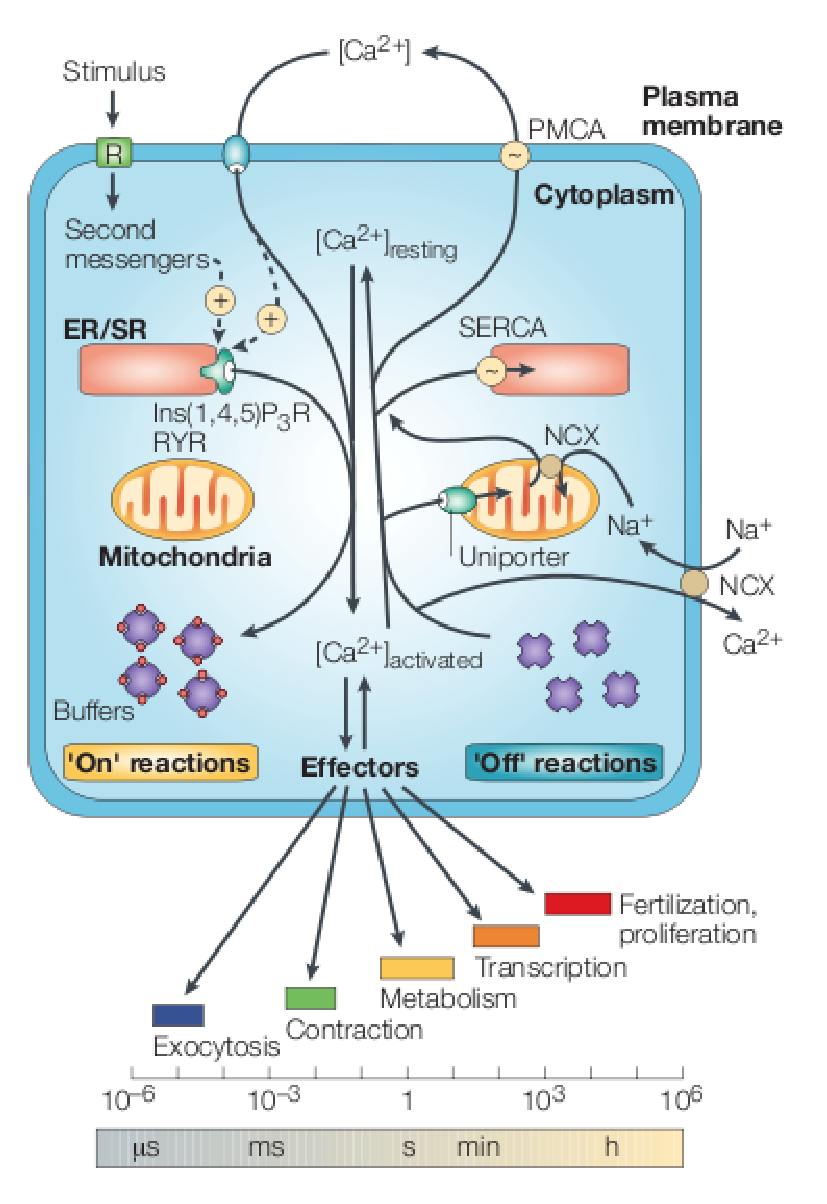
\includegraphics[height=9cm]{./images/calcium_signalling.eps}}
  \caption{\ce{Ca^2+} signalling}\label{fig:Ca_signalling}
\end{figure}







\subsection{Elevated calcium in disease}
\label{sec:calcium-homeostasis-disease}

Alterations in calcium homeostasis are widely reported to contribute to synaptic
degeneration and neuronal loss in Alzheimer's disease
(Sect.\ref{sec:Alzheimer-Disease}).

Elevated cytosolic calcium concentrations lead to activation of the
calcium-sensitive cysteine protease, calpain (Sect.\ref{sec:calpain}), which has
a number of substrates known to be abnormally regulated in disease.


\section{Calcium-binding proteins}
\label{sec:calcium-binding-proteins}
\label{sec:calcium-cells}

Calcium exists as a gradient across the biomembrane, with extracellular
concentration being 4-order of magnitudes higher than intracellular one.
Probably \ce{Ca^2+} is the only molecule with the most widely distributed yet
also very specific in function.

Ca2+ ions function as a diffusible signal that exerts its effect directly or
through {\it calcium-binding proteins} on plasma membrane and intracellular
membranes or in the cytosol. 

% These calcium-binding involved in membrane trafficking,
% and a broad range of enzymes, including kinases, phosphatases, and adenylyl
% cyclases. 

The largest of these families Ca2+-binding proteins sense changes in $[\Ca]$
through either
\begin{enumerate}
  \item 29 a.a. EF-hand motifs -
  Sect.\ref{sec:calcium-binding-proteins-EF-hand}
  
  \item C2 domain (130 a.a.) -
  Sect.\ref{sec:calcium-binding-proteins-C2-domain} 
  
  \item annexins - Sect.\ref{sec:annexin}
%   \item acidic regions of proteins -
%   Sect.\ref{sec:calcium-binding-proteins-acidic-region}
  
  %\item protein-lipid interfaces
\end{enumerate}
Because of this, $\Ca$-binding proteins 

This superfamily has two broad types: 
\begin{enumerate}
   \item A typical structure for $\Ca$ binding site is EF-hand motif -
   Sect.\ref{sec:calcium-binding-proteins-EF-hand}

   \item annexins - Sect.\ref{sec:annexin}
\end{enumerate}

Hence, the calcium indirectly participate in many seemingly unrelated events of
the intracellular signalling system by acting as a diffusible second messenger
to the initial stimuli. Some of the exemplifying events are memory,
contraction-excitation coupling, fertilization...  The calcium-binding proteins
form an intricate network of feedback loops to control the location, amount and
effect of calcium influx.

Even though calcium plays as the second messenger, many of its functions are
indirect, i.e. calcium need to bind to some proteins, and it is these proteins
that do trigger the signal. 

\subsection{A. EF-hand ($\Ca$)-binding proteins}
\label{sec:calcium-binding-proteins-EF-hand}
\label{sec:EF-hand-motif}

A calcium-binding protein has two terminals: C-terminal and N-terminal.
Depending on the type, each terminal (or domain) have a pair of EF-hand
motifs
\begin{enumerate}
  \item C-terminal: slow binding, but bound longer
  
  \item N-terminal: fast binding, but release also quick
\end{enumerate}
The on-rate of $\Ca$ is dependent on the protein; but the off-rate (i.e.
calcium-dissociation) is often much faster in N-terminal (e.g. in CaM $K_d$
= $12.7 \muM$ than in C-terminal (e.g. in CaM $K_d$ = 2.7$\muM$).

An EF-hand motif consists of two alpha helices, "E" and "F", joined by a
Ca(2+)-binding loop. This {\bf helix-loop-helix} structure in EF-hand enables
binding of calcium. EF hands supply an electronegative environment for ion
coordination. After calcium binding, hydrophobic methyl groups from methionine
residues become exposed on the protein via conformational change. X-Ray and NMR
studies shown that conformational changes occured in the
 $\alpha$-helices of EF motif.


EF-hands have been identified in numerous Ca(2+)-binding
proteins. EF-hand homolog family contains more than 160 different
Ca(2+)-modulated proteins which have a broad range of functions. 

Important calcium-binding proteins:
\begin{enumerate}
  \item calmodulin - Sect.\ref{sec:calmodulin}

  Calcium binds to the protein between the C and D helix and also at the
E and F helices (loop). 

  \item troponin-C - Sect.\ref{sec:troponin}
  \item the myosin regulatory light chain, 

  \item the parvalbumin, 
  \item  the S-100 proteins  
  \item the calbindins 9 kDa - Sect.\ref{sec:calbindin}
  \item the calbindins 28 kDa.
\end{enumerate}


\subsection{A.1. neuronal calcium sensors (NCS) family}
\label{sec:neuronal-calcium-sensor}

Neuronal Calcium Sensor (NCS) family of $\Ca$ sensor is a large family of
proteins (with all members have 4 EF-hand motifs). NCS family was originaly
named after a group of proteins that initially thought to be expressed only in
neurons (De Castro et al., 1995). 

NCS are divided into 5 subfamilies based on sequence analysis and order of
theire appearance during evolution:

\begin{enumerate}

  \item class A: {\bf frequenin}/NCS-1  (found first in yeast)
  
  \item class B: {\bf VILIP} (visinin-like protein) - found first in {\it C.
  elegans} - Sect.\ref{sec:VILIP}
  
  \item class C: {\bf recoverin} - Sect.\ref{sec:recoverin}
  
  \item class D: {\bf GCAP} (Sect.\ref{sec:GCAP}) - found in vertebrate
  
  \item class E: {\bf KChIP} - found in vertebrate - Sect.\ref{sec:KChIP}
\end{enumerate}

\textcolor{red}{In mammals, the genome has one type NCS-1, five VILIPS
(hippocalcin, neurocalcin-$\delta$, VILIPs1-3), one type recoverin, and three
GCAPs (GCAP1-3), and four types of KChIP (KChIP1-4).}

All the members of NCS, except KChIP2 and KChIP3, show N-terminal myristoylation
concensus sequence. $\Ca$ binding are generally cooperative, and also
the affinities for calcium in the members are much higher compared to that in
calmodulin; even though the expression level is lower. This poses the question
of so-called ``calcium race''? - {\bf how NCS family members can get
calcium, when CaM is dominated, to perform its function?}

% which work as calcium dependent molecular switches and includes
% members like Frequenin (NCS1), recoverin, GCAP, neurocalcin, visinin, etc.


\subsection{---- NCS-1 (neuronal calcium sensor-1, frequenin)}
\label{sec:NCS-1}
\label{sec:frequenin}

Neuronal calcium sensor-1 (NCS-1) also known as {\bf frequenin} homolog
(Drosophila) (freq) (as was originally discovered in Drosophila as a
gain-of-function mutation associated with frequency-dependent increases in
neurotransmission) is the member of neuronal calcium sensor family.

\textcolor{red}{WARNING}: The designation 'NCS-1' came from the assumption that
the protein was expressed only in neuronal cell types, which is not the case.

\textcolor{red}{In diseases}:
The expression of NCS-1 increases in bipolar disorder and some forms of
schizophrenia; while decreases in  inflammatory bowel diseases. NCS-1 has also
been linked with Autism. NCS-1 is significant in intelligence in creating
curiosity by its function on dopamine D2 receptors in the dentate gyrus,
increasing memory for complex tasks.

Ca(2+)/NCS-1 has roles:
\begin{enumerate}
  \item bind to D2-receptor in dentate gyrus: 
  
   two copies of the D2R peptide bind within the hydrophobic crevice on
  Ca(2+)/NCS-1 in that the  C terminus and EF3-EF4 linker of NCS-1
  modulate binding (Pandalaneni et al., 2015)
  \url{https://www.ncbi.nlm.nih.gov/pubmed/25979333}
  
  \item bind to cognate kinases GRK1 and GRK2 - Sect.\ref{sec:GRK}.
  
  only one copy of the GRK1 peptide binds Ca(2+)/NCS-1
   
\end{enumerate}

\subsection{---- VILIP}
\label{sec:VILIP}

There are five VILIPS (hippocalcin, neurocalcin-$\delta$, VILIPs1-3) in
mammalian genomes. 
\begin{enumerate}
  \item hippocalcin - Sect.\ref{sec:hippocalcin}
\end{enumerate}

\subsection{------ hippocalcin}
\label{sec:hippocalcin}

{\bf Hippocalcin} is a $\Ca$-binding protein expressed in neurons (especially
in the hippocampus), i.e. belongs to neuronal calcium sensor (NCS) family in
particular VILIP (class B) subfamily - Sect.\ref{sec:VILIP}.

Its functional role
\begin{enumerate}
  \item inhibition of apoptosis - Sect.\ref{sec:apoptosis}
  
  Hippocalcin interacts with NAIP (neuronal apoptosis inhibitory protein) -
  Sect.\ref{sec:NAIP}
  
  \item MAP-kinase signaling
  
  \item LTD in hippocampal neuron
  
  \item required for normal spatial learning
  
  \item activate PLD1 and PLD2 expression  - Sect.\ref{sec:PLD}
\end{enumerate}

\subsection{---- GCAP: guanylate cyclase activating protein}
\label{sec:GCAP}

GCAP (guanylate cyclase activating protein)

\subsection{---- recoverin (23 kDa): in eye}
\label{sec:recoverin}

{\bf Recoverin} (23 kDa) is a neuronal $\Ca$-binding protein
primarily found in {\bf photoreceptor cells of the eye}.

Its role in 
\begin{enumerate}
  \item inhibiton of rhodopsin kinase - the enzyme that regulate
  phosphorylation of rhodopsin - Sect.\ref{sec:rhodopsin-like-GPCR}
  
 Activation of recoverin controls the life span of photoexcited rhodopsin by
 helping to inhibit rhodopsin kinase, resulting in the prolongation of light
 sensitivity for rhodopsin.
 
 Light-dependent channel closure in photoreceptors causes calcium levels to
 decrease, which relieves the inhibition of rhodopsin kinase by calcium-bound
 recoverin, leading to a more rapid inactivation of metarhodopsin II (activated
 form of rhodopsin).
  
  \item light-dependent intracellular translocation to rod synaptic terminals
  and improves the signal transfer between rods and rod bipolar cells in the
  retina of mice 
\end{enumerate}


\subsection{---- KChIP}

Check sect.\ref{sec:KChIP} for details.


%\subsection{c. acidic region}

\subsection{A.2. (neuronal) Calcium-binding protein (CaBP and nCaBP)}

Unlike NCS family (Sect.\ref{sec:neuronal-calcium-sensor}), neuronal
calcium-binding protein (nCaBP) family arose much later during evolution and are
found only in vertebrate.   The function of neuronal $\Ca$-binding proteins
(NCBP, nCaBP) is largely unknown.

nCaBP family includes

\begin{itemize}

  \item {\bf caldendrin/CaBP 1-5 isoforms} - Sect.\ref{sec:CaBP1-CaBP5}
  
  \item {\bf calneurons-1 and -2} (sect.\ref{sec:calneurons}): also known as
  CaBP7 and CaBP8.
  
  Calneurons-1 and -2 evolved independently from caldendrin/CaBP with a
  different EF-hand organiation. In particular, \textcolor{red}{calneurons have
  higher calcium-binding affinities and carboxyl-terminal transmembrane domain}.
  Though, they are assigned to CaBP family due to mainly sequence similarity.
\end{itemize} 

The EF-hands in nCABP show much similarity of those in calmodulin; than to NCS
family. Also, there are 4 extra amino acids in the linker regions between two
EF-hand pairs in calendrin/CaBP (Haeseleer et al., 2000). \textcolor{red}{NOTE:}
two members (CaBP1 and CaBP2) also have {\bf N-myristoylated}.

\subsection{---- CaBP1 - CaBP5}
\label{sec:CaBP1-CaBP5}

CaBP family has 5 members (CaBP1, CaBP2, CaBP3, CaBP4, CaBP5) identified in
vertebrate retina; whose sequences show 46-58\% similarity to CaM. The
difference to CaM:
\begin{enumerate}
  \item  alterations within their second EF-hand loop inactivate in $\Ca$
  coordination
  
  \item central $\alpha$-helices are extended by one $\alpha$-helical turn. 
\end{enumerate}

NOTICE: In reconstitution assays, CaBPs are able to substitute functionally for
CaM - Sect.\ref{sec:calmodulin}).
\begin{enumerate}
  \item CaM-like CaBP: the shortest (149-150 a.a.; and about 16.8 kDa)
  
  \item other members: about 200 a.a. long; and about 23 kDa molecular mass. 
\end{enumerate}

\subsection{------ CaBP1 (caldendrin, CDD/CaBP1)}
\label{sec:caldendrin}
\label{sec:CDD-CaBP1}


{\bf Calcium-binding protein 1} (caldendrin, or CDD/CaBP1) is a protein, (in
human) is encoded by {\it CABP1} gene. The protein is discovered in 1999; with 2
EF-hand motifs.

CaBP1 and CaBP2 are expressed as multiple, alternatively spliced variants, and
in heterologous expression systems these forms show different patterns of
subcellular localization. 

CABP1 is expressed in {\bf neuronal cells} (in cerebral cortex, hippocampus,
habenular nucleus of epithalamus - Sect.\ref{sec:epithalamus}, Purkinje cell
layer of cerebellum, and retina (amacrine cells and cone bipolar cells)).


\subsection{------ Calcium-binding protein 5 (CaBP5)}
\label{sec:CaBP5}

CaBP5 is found  restricted to retinal rod and cone bipolar cells.

\subsection{---- calneurons}
\label{sec:calneurons}



\subsection{-- S-100 proteins: S100A1, S100A2, S100A3}
\label{sec:calcium-binding-proteins-acidic-region}
\label{sec:S100A}

Considering the importance of negative surface charges for calcium binding
(Linse et al., 1988), the S-100 proteins are a group of small acidic Ca2+
-binding proteins that are expressed in a cell-type-dependent fashion (review:
Kligman and Hilt 1988). Later, it is recognized that these S-100 proteins has 2
calcium-binding site that have EF-hand type conformation.

These proteins have sequence similarity with calmodulin and other
calcium-binding proteins (Moore 1965; Calissano et al. 1969; Dannies and Levine
1971; Isobe et al. 1977; Isobe and Okuyama 1978 and 1981). Unlike Calmodulin
which is a ubiquitous proteins, the distribution of particular S-100 proteins
appears to be restricted to specific cell types (Hilt, Kligman, 1991 - book
chapter of the book ``Novel-calcium binding proteins" edited by Wasserman
(1991)), and depends on environmental factors.
\begin{enumerate}
  \item S100A1

S100 calcium-binding protein A1 is highly expressed in cardiac, skeletal muscle,
and localized to cytoplasm at Z-discs and sarcoplasmic reticulum (SR).
It is a potential target for gene therapy to treat post-myocardially infarcted
cardiac tissue.

  \item S100A2

  \item S100A3

\end{enumerate}




\subsection{B. C2 domain}
\label{sec:calcium-binding-proteins-C2-domain} 

The C2 domain was originally identified as the second of four conserved domains
(C1 though C4) in the conventional type of PKC, i.e. (c)PKC, at $\alpha$,
$\beta$ and $\gamma$ isoforms - Sect.\ref{sec:PKC-isoforms}.
The core structure of the C2 domain is based entirely on beta-sheets rather than
on alpha-helices.

\subsection{-- Synaptogamin-2}
\label{sec:synaptogamin-2}

Synaptogamin family is characterized by two C-terminal calcium-binding motifs
(Sect.\ref{sec:calcium-binding-proteins-C2-domain}), is expressed throughout the
brain .
Synaptotagmin 1 and 2 (syt 1, syt 2) are synaptic vesicle-associated membrane
proteins that act as calcium sensors for fast neurotransmitter (Fox, Sanes,
2007).

Synaptotagmin-2  is a protein that shows calcium-dependent phospholipid and
inositol polyphosphate binding. It binds 3 $\Ca$ ions per subunit, at
C2-domain .

Syt 1 and syt 2 are localized predominantly to different subsets of
synapses in retina, hippocampus, cerebellum, and median nucleus of the trapezoid
body (MNTB). Syt2 triggered release with shorter latency and higher temporal
precision and mediated faster vesicle pool replenishment than Syt1.

The distribution is spatial and temporal difference
\begin{enumerate}
  \item In the MNTB, syt 1 and syt 2 are present in different presynaptic
  terminals on the same postsynaptic principal neuron.
  
  \item In retina, horizontal and OFF-bipolar cell terminals contain syt 2,
  whereas most other terminals contain syt 1.
  
Syt 1 localization in the immature retina resembles that seen in adult; however,
syt 2 localization appears strikingly different at perinatal ages and continues
to change dramatically prior to eye opening.  

  \item species-specific differences in synaptotagmin localization were observed
  in retina and cerebellum

  \item Syt 1:  synaptotagmin 1 (Syt1) was enriched in excitatory terminals

  
  \item Syt 2 (fast-release of neurotransmitter at inhibitory synapse):  In
  presynaptic side of inhibitory nerons, the AP is typically short, i.e.
  short-lived calcium spike. So, how to sense $\Ca$ to enable the release of
  GABA neurotransmitter? Syt2  seems to act as $\Ca$ sensor of exocytosis at
  GABAergic basket cell (BC) to Purkinje cell (PC) synapses in cerebellum.
  
  Genetic elimination of Syt2 reduced action potential-evoked release to
  only 10\%, identifying Syt2 as the major Ca2+ sensor at BC-PC synapses (Chen
  et al., 2017).

 NOTE: at two types of fast-releasing inhibitory connections in the mammalian
 CNS: the medial nucleus of the trapezoid body to lateral superior olive
 glycinergic synapse, and the basket/stellate cell-Purkinje GABAergic synapse  
 in the cerebellum. They showed that Syt1 is weakly expressed; yet must be
 genetically inactivated together with Syt2 to achieve a significant reduction and
   desynchronization of fast release (Bouhours et al., 2017). 
\end{enumerate}

\url{http://www.uniprot.org/uniprot/Q8N9I0}

\subsection{C. annexins}
\label{sec:annexin}

The term {\bf annexins} refers to calcium- and phospholipid-binding proteins
that can aggregate to membrane in a calcium-dependent manner.
Annexins (ANX) are a large family of calcium-dependent membrane-binding
proteins, mainly found in  eukaryotes but largely absent in prokaryotes and
yeasts. Each protein contains conserved internal 4 to 8 tandem repeats of about
60-80 amino acids each (Weinman, 1991). All these repeats include a highly
conservative 17-member amino acid consensus sequence (an endonexin fold).
% \url{https://www.ncbi.nlm.nih.gov/pubmed/1864864}

\begin{mdframed}
Annexins are devoid of the classical "EF-hand" Ca(2+)-binding domain and can
therefore be assigned to a new family of Ca(2+)-binding proteins (Melgunov,
1991). The Ca2+-binding sites of annexins differ fundamentally from the EF-hand
arrangement, because only five of the seven coordination sites are provided by
protein oxygens and because no EF-hand-type helix-loop-helix structure is discernible. 

\end{mdframed}


The first protein of this family, {\bf synexin} (now is known as {\it annexin
A7}, was found in 1977. Synexin (from the Greek: synexis), which means
"meeting". The descriptor 
\begin{itemize}
  \item  'A' denotes their presence in vertebrates; 
  
  \item 'B' denotes  their presence in invertebrates; 
  
  \item 'C' denotes their presence in fungi and some groups of unicellular
  eukaryotes; 
  
  \item 'D' denotes their presence in plants; and 
  
  \item 'E' their presence in protists   
\end{itemize}

More than a 100 annexins have been identified in many different species: 12
annexins were found in human (annexins A1-A13; no counting A12 which is
unassigned);  Zebrafish have eleven annexin genes. NOTE: three zebrafish ANX
genes are homologous with human ANX1; two are homologous with human ANX2; and
two are homologous with human ANX11  (review: Mirsaeidi et al., 2016)

In human: 
\begin{enumerate}
  \item  annexin A7 (synexin):  caused aggregation (in a temperature-dependent
  manner) of chromaffin granules in the adrenal glands in the presence of free
  calcium
  
  It did not cause granule aggregation in the presence of magnesium, barium, or
  strontium, but was activated by calcium.
  
  \item 
\end{enumerate}


%https://www.ncbi.nlm.nih.gov/labs/articles/1873340/

\begin{enumerate}
  \item 35 kDa annexins: contains 4 repeats
\end{enumerate}

\section{Calpain (calcium-activated protease)}
\label{sec:calpain}

In 1964, a calcium-activated protease (Sect.\ref{sec:protease}) - enzyme that
breakdown proteins and peptide - were detected in brains, lens of the eye, and
other tissues.

In late 1960s, this enzyme was isolated, and characterized (in both rat brain
and skeletal muscle) as activated at neutral pH.

In 1984, when the enzyme was sequenced, it was given the name {\bf calpain} as
the hybrid of two well-known proteins at the time, the calcium-regulated
signalling protein, {\bf cal}modulin, and the cysteine protease of papaya,
pa{\bf pain}.

In 2002, calpain was classified into 
\begin{enumerate}
  \item $\mu$(mu)-calpain - Sect.\ref{sec:mu-calpain}: activated at micro-molar
  range of $\Ca$

  \item m-calpain - Sect.\ref{sec:m-calpain}: activated at mili-molar range of
  $\Ca$
 
\textcolor{red}{In the brain, while $\mu$-calpain is mainly located in the cell
body and dendrites of neurons and to a lesser extent in axons and glial cells,
m-calpain is found in glia and a small amount in axons. }

\end{enumerate}
The Human Genome Project has revealed that there are more than a dozen other
calpain isoforms, some with multiple splice variants.

\subsection{mu-calpain (calpain 1)}
\label{sec:mu-calpain}
\label{sec:calpain-1}

$\mu$-calpain (calpain 1) is activated at micro-molar range of $\Ca$.

\subsection{m-calpain (calpain 2)}
\label{sec:m-calpain}
\label{sec:calpain-2}


\begin{mdframed}

Calpain activation was monitored by quantitative analysis of spectrin
degradation and by a FRET-based assay, which assessed the truncation of a
calpain-specific peptide flanked by the FRET fluorophore pair, DABCYL and
EDANS (Jourdi et al. (2010)).
%https://www.ncbi.nlm.nih.gov/pmc/articles/PMC2820881/
\end{mdframed}

m-calpain (calpain 2) is activated 
\begin{enumerate}
  
  \item at mili-molar range of  $\Ca$, or
  
  \item (in fibroblasts) epidermal growth factor (EGF - Sect.\ref{sec:BDNF}) can
  activate m-calpain independently of calcium via mitogen-activated protein kinase (MAPK)-mediated
  phosphorylation 

  \item (in neurons): indirectly via BDNF - see MAPK/ERK pathway
  (Sect.\ref{sec:MAPK/ERK-pathway}), and preferentially localized to dendrite
  and dendritic spines.
 
\end{enumerate}


\subsection{functions}

A transient and localized influx of calcium into the cell activates a small
local population of calpains (for example, those close to Ca2+ channels), which
then advance the signal transduction pathway by catalyzing the controlled
proteolysis of its target proteins.

\url{https://en.wikipedia.org/wiki/Calpain}






\section{Calcium spikes (oscillations) and waves}
\label{sec:calcium-oscill-waves}
\label{sec:calcium-oscillation}
\label{sec:calcium-spike}

Betwen calcium spike and calcium oscillation, the term {\bf calcium spike} is
preferred as spikes evoke the image of a process with a sharp threshold, an
explosive rise, and an amplitude independent of stimulus intensity. Spikes are
driven by positive feedback. In contrast, oscillations can be generated by
negative feedback alone. The heart of a spiking mechanism is its
positive-feedback loop (Stryer, Myer, 1991).

Spiking emerges from bistability (Sect.\ref{sec:bistability}) which requires
cooperativity and positive feedback. However, another important properties
required are deactivation and reactivation.
\begin{enumerate}
  \item de-activation: means reduced in calcium-uptake into the IP3-insensitive
  pool, such as mitochondria; and also Calcium-inhibition calcium release by
  blocking IP3R.
  
However, in cells such as RBL, calcium spiking is not prevented by inhibitors
that prevent calcium entry into mitochondria. 

Another deactivation mechanism is $\Ca$ blocking IP3R.
This inhibition is an attractive deactivation mechanism because it directly
senses the spike height.
So, calcium ions play dual role: positive feedback to IP3 production (via
activation of PLC), and blocking effect of IP3 on calcium release (via
inhibiting IP3R)
 
  \item 
\end{enumerate}

In many cell types, the strength of the extracellular stimulus is encoded
primarily in the frequency of the cytosolic [$\Ca$]$_c$ oscillations, which
increases with the degree of stimulation.
\begin{enumerate}
  \item IP3-dependent pathway - Sect.\ref{sec:IP3-calcium-oscillation}
  
\end{enumerate}

The calcium release can occur in complex spatial patterns, especially waves.
\textcolor{red}{Calcium waves, the spatial counterpart of calcium spiking, have
also been detected in many cells}. These propagating calcium waves are thought
to have functional significance in different cellular events, e.g. establishing
polarity in eggs at fertilization \citep{gilkey1978}, directing fluid secretion
across epithelial cells \citep{kasai1990}.

Calcium spikes have been observed in
\begin{enumerate}
  \item hepatocytes 
  \item fibroblasts
  \item T lymphocytes
  \item neutrophils
  \item adrenal glomerulosa cells
  \item pituitary cells
  \item pancreatic acinar cells
  \item insulinoma cells
\end{enumerate}

Calcium waves have been observed using either aequorin
(Sect.\ref{sec:aequorin}) or a fluorescent indicator (Sect.\ref{sec:fluorescence-dyes}) in
such large cells as
\begin{enumerate}
  \item  oocytes (25, 46, 48), 
  
  \item myocytes (69), 
  
  \item astrocytes ( 1 6), and

  \item hepatocytes
\end{enumerate}

\subsection{Properties} (Myer, Stryer, 1991) 

\begin{enumerate}
  \item Spiking occurs at a sharp threshold. Cai is virtually unaltered by subthreshold
levels of hormones and other agonists.

  \item The frequency of spiking is approximately proportional to the
  concentration of agonist over a considerable range (typically 3- to 1 0-fold).

Very high agonist concentrations lead to a sustained elevation of Cai
rather than to spiking
  
  \item The latency of the calcium response (the interval from addition of
agonist to the first spike) decreases with increasing agonist concentration.

  \item For a given agonist, the rise time, amplitude, and duration of spikes
are nearly independent of agonist concentration

This invariance reveals that spikes are produced by excitation of bistable
systems. Sharp thresholds and concentration-dependent latencies are additional
manifestations of bistability

  \item Bistable systems support wave propagation. Calcium waves are the
counterpart in space of calcium spiking in time. The velocity of calcium
waves ranges from 5 to 100 $\mu$m/s.

  \item The rise time of a spike is typically 1 s and the duration is several
seconds

The interval between spikes is usually between a few seconds and a minute,
depending on the particular agonist and its concentration.

  \item  Many cells can undergo spiking for a limited time in the absence
of extracellular Ca2+, showing that the source of Ca2+ is
intracellular.

The corollary is that membrane potential does not influence spiking in cells
lacking voltage-gated calcium channels.

  \item  Activation of protein kinase C (PKC) increases the threshold for spiking
and lowers the spiking frequency, as evidenced by the effect of adding phorbol
esters. 

Phosphorylation by PKC desensitizes the calcium response, most likely by
blocking G-protein stimulation of phospholipase C.
  
  \item Different agonists induce distinguishable spike patterns, implying
that two or more pathways that control or modulate Cai are differentially
stimulated.

Generally, each cell has a calcium fingerprint - it sings its own calcium song
with distinctive spiking patterns.

\end{enumerate}

The essential ingredients for bistability are positive feedback and
cooperativity (Sect.\ref{sec:bistability}). What molecular events in calcium
spiking correspond to positive feedback, cooperativity, deactivation, and
reactivation?

\subsection{Non-excitable cell}
\label{sec:calcium-oscillation-non-excitable-cell}

IP3R is the main type of ER calcium release channel in nonexcitable cells
(Sect.\ref{sec:IP3-calcium-oscillation}). The existence of calcium oscillation
(Sect.\ref{sec:calcium-oscill-waves}) in non-excitable cells was first suggested
by \citep{prince1973}, in that the flucutation of internal calcium is due to
periodic release of $\Ca$ from ER, stimulated by IP3.

The role of \IPthree as a frequency-coded second messenger in regulating calcium
in non-excitable cells are well-defined \citep{woods1986, thomas1996}. 

Later on, it was observed the first time on hepatocytes using aequorin by
\citep{woods1986, woods1987}.  The addition of physiologic concentrations of
vasopressin, a hormone known to mobilize intracellular calcium, gave a
surprising result. A sustained rise in Caj was expected, but, instead,
repetitive increases in calcium (calcium spikes) occured from basal level
200$\muM$ to peak 1 $\muM$, each spike lasts about 7 seconds. In hepatocytes of
stressed animal, the vasoactive hormones vasopressin and angiotensin-II and the
neurotransmitter noradrenaline induce liver cells to release glucose from
glycogen (Sect.\ref{sec:glyocogenolysis}). The mechanism is that the hormones
bind to cell-surface receptors (inositol lipid-specific phospholipase (PLC))
which then induce the hydrolis of phosphatidyl-inositol 4,5-biphosphate(a minor
plasmalemma lipid), to produce \IPthree and diacylglycerol.

\begin{enumerate}
  
  \item {\bf hormones}: in rat hepatocytes, the periods of [Ca2+]c oscillations
  range over one order of magnitude, from 250 sec for low concentrations of
  hormones, such as vasopressin and noradrenalin, to 30 sec for higher hormone
  doses (Rooney et al., 1989).

%   Rooney, T., E. Sass, and A. P. Thomas. 1989. Characterization of
% cytosolic calcium oscillations induced by phenylephrine and vasopressin
% in single fura-2-loaded hepatocytes. J. Biol. Chem. 264:17131-17141.

Hormones that act through the calcium-releasing messenger, inositol
1,4,5-trisphosphate (IP3), cause intracellular calcium oscillations.

% Rooney, T., E. Sass, and A. P. Thomas. 1989. Characterization of cytosolic
% calcium oscillations induced by phenylephrine and vasopressin in single
% fura-2-loaded hepatocytes. J. Biol. Chem. 264:17131-17141.

  \item {\bf antigen}: activate T lymphocytes (human T-leukemia-derived line,
  Jurkat) - (Lewis \& Cahalan, 1989)
  
Phytohemagglutinin (PHA), a mitogenic lectin, in- duces repetitive [Ca2]i
oscillation at peak of micromolar levels with a period of 90-120 sec.
The oscillations depend critically upon Ca2+ influx across the plasma membrane.
  
  \item It's known that calcium oscillation regulates contraction in smooth muscle
\citep{bai2009, sanderson2010}, via an RyR-independent and IP3-dependent pathway
(Sect.\ref{sec:smooth-muscle-small-airways}).

\end{enumerate}

% 6. Keizer, J., Y. X. Li, S. Stojilkovic, and J. Rinzel. 1995. InsP3-induced Ca2+
% excitability of the endoplasmic reticulum. Mol. Biol. Cell. 6:945-951.
% 
% 7. Dupont, G., S. Swillens, C. Clair, T. Tordjmann, and L. Combettes.
% 2000. Hierarchical organization of calcium signals in hepatocytes:
% from experiments to models. Biochim. Biophys. Acta. 1498:134-152.
% 
% 8. Schuster, S., M. Marhl, and T. Ho¨ fer. 2002. Modelling of simple and
% complex calcium oscillations. From single-cell responses to intercellular
% signaling. Eur. J. Biochem. 269:1333-1355.

\subsection{Excitable cells}
\label{sec:calcium-oscillation-excitable-cell}



\subsection{IP3-dependent}
\label{sec:IP3-calcium-oscillation}

Sect.\ref{sec:ip3-pathways} describes the mechanisms, as well as level of
calcium and IP3 for IP3 receptor gating. IP3-dependent of $\Ca$ oscillations is
first observed in non-excitable cells
(Sect.\ref{sec:calcium-oscillation-non-excitable-cell})

\label{sec:IP3-oscillation-mechanisms} Several mechanisms have been proposed to
explain oscillations of intracellular Ca2+ concentration in nonexcitable cells.

\begin{enumerate}
  \item IP3-mediated $\Ca$ release and $\Ca$-activated PLC - 
  Sect.\ref{sec:calcium-oscillation-Ca-activated-PLC}

Here, oscillation can be produced without any requirement of IP3R regulation by
$\Ca$ (i.e. inactivation). However, it requires IP3 oscillations.
However, it is experimentally observed that calcium oscillation can be
reproduced using (Wakui et al., 1989)

% Wakui, M., B. V. Potter, and O. H. Petersen. 1989. Pulsatile intracellular
% calcium release does not depend on fluctuations in inositol trisphosphate concentration
%Nature. 339:317-320.
  
  \item 
\end{enumerate}

\subsection{-- feedback of IP3/DAG on PLC, upstream GTP/GPCR (simple IP3R
dynamics)}
\label{sec:calcium-oscillation-Ca-activated-PLC}

IP3 injected into intact cells evokes irregular and transient oscillatory
$\Ca$-dependent current responses, i.e. $\Ca$-dependent $\Cl$ current; and in
such experiments, level of IP3 are not constant.

Beside fluctuating level of IP3 as a key component in generating calcium
oscillation, the 'receptor-controled $\Ca$ oscillation hypothesis' types of
models was developed to account for the striking dependence of calcium
oscillations (particular the shape and duration of free calcium transients) on
the receptor type; which is modeled via the
\begin{enumerate}
  \item rate of conversion between G$\alpha$-GDP and G$\alpha$-GTP
  \item rate of PKC phosphorylation on G$\alpha$-GTP
\end{enumerate}

Such mechanism (e.g. induced by insulin) is suggested on {\bf
non-excitable cells} (hepatocyte, endothelial cell); assuming that $\Ca$ influx
are not directly involved in calcium oscillations (experiments with reduced
$[\ca]_o$ also found oscillations, suggest the dependency on calcium entry is
more indirect in these cells).

\begin{itemize}
  \item model for hepatocyte : Cuthbertson - Chay (1991)

Cobbold et al. first showed that a constant agonist concentration could evoke
repetitive $\Ca$ spikes in hepatocytes (Woods et al., 1986). Stimulation of
cell-surface recptors (G-coupled protein receptors) initiate an IP3-dependent
pathway of $\Ca$ oscillation - Sect.\ref{sec:GPCR-PLC-IP3-DAG-pathway}.
% Woods, Cuthbertson, Cobbold (1986) Nature

In these models, calcium oscillations can be generated via IP3-mediated Ca2+
release coupled to Ca2+-activated PLC (Sect.\ref{sec:PLC-Calcium}) can generate
oscillations, without any requirement of IP3R regulation by Ca2+.

Simple IP3-mediated IP3R dynamics (e.g. no inhibition) generally produce
[Ca2+]c oscillations with short periods (;10-60 s) and thus do not reproduce the
long interspike intervals observed experimentally.

  \item 
\end{itemize}

These models have been criticized because in some cell types Ca2+ oscillations
can also be elicited by IP3 or its nonmetabolizable analogs.


NOTE:
\begin{enumerate}
  \item  the build-up of GTP-bound G$\alpha$ subunits, 
  combined with positive feedback process (via DAG enhancing PLC actiation) and
  perhaps cooperative effects (e.g. $n=2$ DAGs binding is required for
  enhancing PLC activation), lead to the sudden activation of PLC, eventualy
  $\Ca$ elevation.
  
All PLC isoforms are activated by Ca2+ ions, although their sensitivities to
[Ca2+] vary greatly.

  
  \item the negative process (via PKC), which is hypothesied by the reducing in
  the pool of GTP-bound G$\alpha$ subunits, switches off $\Ca$ rise and lead to a fall in
  $\Ca$ level.
  
  Two proposed negative feedback mechanisms
  \begin{itemize}
    \item  phosphorylation by PKC of GPCR (at $\alpha$ subunit), i.e. making
    the receptor less sensitive to ligands
    
    \item stimulation of GTPase activating factor (GAF) activity
    (Sect.\ref{sec:GAF-domain}) by activated PLC (Sect.\ref{sec:PLC})
    
    Activated GAF the hydrolyze G$\alpha$-GTP to G$\alpha$-GDP
  \end{itemize}
  
\end{enumerate}



\begin{verbatim}
NOTE: Ga-GTP = GTP-bound G-protein

agonist -[bind GPCR]-> Ga-GTP --[Ca2+]-> PLC 
   PLC -[cleave PIP2]-> IP3 + DAG 
   IP3 --> IP3R --> Ca2+ 
   PKC --[DAG]--> PKC*
   GPCR --[PKC*]---> GPCR_desensitized
   GAF --[PLC]---> GAF*
   Ga-GTP --[GAF*]--> Ga-GDP

 Ca2+ (positive feedback to PLC)
 PKC* (negative feedback)
 PLC* (negative feedback)
\end{verbatim}

$\Ca$ oscillations can occur when IP3 concentration is held at a constant value.
However, computational models based on this simple description of the IP3R
dynamics generally produce [$\Ca$]c oscillations with short periods (about 10-60
s) and thus do not reproduce the long interspike intervals observed
experimentally. 

\subsection{-- threshold of PLC activation for spiking}

The existence of a threshold for spiking ensures that a low degree of activation
of PLC does not raise the cytosolic calcium level.
PLC activation requires G$\alpha$-GTP and $\Ca$ (Sect.\ref{sec:PLC-Calcium}).

A cell can ignore subthreshold stimuli or noise induced by components of the
transduction chain. (Meyer - Stryer, 1988). Also, the rare fluctuation that
triggers a single spike is unlikely to persist and lead to a train of spikes.

A single messenger such as calcium could excite different effector systems
depending on the spike frequency. Cooperatively activated calcium-binding
proteins, such as calmodulin, are well suited for detecting calcium spikes
because they can be designed to be switched on only at spike peaks.




\subsection{-- phosphorylation of IP3R regulation by Ca2+}

Calcium oscillation has also been observed under fixed (constant) IP3 level
in mouse pancreatic acinar cells (Wakui et al., 1989)
\begin{itemize}
  \item Single internally perfused mouse pancreatic acinar cells: Acetylcholine
  (ACh) acting on muscarinic receptor
  (Sect.\ref{sec:muscarinic-acetylcholine-receptor}) evoke regular and
  repetitive current pulse, via $\Ca$-activated $\Cl$ current
  
  To fix IP3, it is replaced by non-metabolizable InsP3 analogue {\bf Inositol
  trisphosphorothioate} (InsPS$_3$). IPS$_3$ is 3x less potent to IP3R than IP3;
  yet it is resistant to metabolism via 5-phosphatase pathway and 3-kinase
  pathway (Sect.\ref{sec:IP3-degradation}).
\end{itemize}


More complex mechanisms of IP3R can help to explain long cycle $\Ca$
oscillations. Long-period oscillations have been obtained when additional
mechanisms, such as the regulation of IP3R by phosphorylation, stochastic gating
phenomena or slow calcium buffers, are included

% 9. Sneyd, J., K. Tsaneva-Atanasova, J. I. Bruce, S. V. Straub, D. R.
% Giovannucci, and D. I. Yule. 2003. A model of calcium waves in
% pancreatic and parotid acinar cells. Biophys. J. 85:1392-1405.
% 
% 10. Falcke, M. 2003. On the role of stochastic channel behavior in intracellular
% Ca2+ dynamics. Biophys. J. 84:42-56.
% 
% 11. Marhl, M., T. Haberichter, M. Brumen, and R. Heinrich. 2000.
% Complex calcium oscillations and the role of mitochondria and
% cytosolic proteins. Biosystems. 57:75-86.


Yule and Bruce (2003) 

\begin{verbatim}
agonist -[bind GPCR]-> GTP-bound G-protein --[Ca2+]-> PLC 
   PLC -[cleave PIP2]-> IP3 + DAG 
   IP3 --> IP3R --> Ca2+ 
    
 Ca2+ (positive feedback to PLC)
 Ca2+ (negative feedback: inhibit IP3R at high-concentration)
 IP3R has 2 Ca2+ binding sites (one activation, and one inactivation)
\end{verbatim}
\ref{sec:IP3R}

\subsection{-- IP3R regulation: fast activation and delayed inhibition of RyR}


Mathematical models have demonstrated how fast activation and delayed inhibition
of the IP3R by cytoplasmic Ca2+ can drive repetitive Ca2+ spiking
Therefore, Ca2+ oscillations can occur when IP3 concentration
is held at a constant value.


\subsection{-- IP3 oscillations }
\label{sec:calcium-oscillation-IP-oscilate}

In the previous models
\begin{itemize}
  \item Models based on a simple description of the IP3R dynamics generally produce
[Ca2+]c oscillations with short periods (10-60 s) and thus do not reproduce the
long interspike intervals observed experimentally.
  
  \item Long-period oscillations have been obtained when additional mechanisms, such as
the regulation of IP3R by phosphorylation, stochastic gating phenomena or slow
calcium buffers, are included (review: Politi et al. 2006). 
%   \item  Long-period oscillations have been obtained when additional mechanisms, such as
% the regulation of IP3R by phosphorylation, stochastic gating phenomena or slow
% calcium buffers, are included (review: Politi et al. 2006).

\end{itemize}
\textcolor{red}{However, the question is 'is this the efficient frequency
encoding of hormone dose?'}

Here, it is suggested that IP3 oscillations may underlie efficient frequency
encoding of the hormone signal. The existence of both positive and negative
feedbacks of Ca2+ on IP3 metabolism could mediate fluctuations in cellular IP3
levels (Sect.\ref{sec:IP3-oscillation-mechanisms}).

The existence of both positive and negative feedbacks of Ca2+ on IP3 metabolism
could mediate fluctuations in cellular IP3 level (Sect.\ref{sec:IP3_synthesis}).
Modeling has suggested that the lifetime of IP3 is a critical parameter in the
system (Politi et al., 2006).


% \begin{enumerate}
% 
% 
%   \item Politi et al. (2006) showed that a coupled IP3- -Ca2+ oscillator may generate
% long-period oscillations and underlie the efficient frequency encoding of the
% hormone dose.
% 
% 
%   \item 
% \end{enumerate}


\begin{enumerate}

  \item $\Ca$-induced $\Ca$ release
  
  \item agonist-receptor mediated by G proteins, DAG, PKC
  
  \item positive feedback and negative feedback of $\Ca$ on the production of
  IP3 through PLC (Sect.\ref{sec:PLC}).
  
  \item biphasic responses of IP3R to cytosolic calcium (maybe sufficient to
  induce $\Ca$ oscillations). The oscillations occurs when $\ca$ provides a
  feedback upon the production rate of IP3 through PLC
  (Sect.\ref{sec:IP3_synthesis}).

Extravesicular of $\Ca$ near microsomal vesicles where $\Ca$ are released can
increase from 100 nM to 100 $\muM$.
\end{enumerate}






%\section{Calcium waves}

\section{Calcium storage}


In vertebrates, \ce{Ca^2+} is mainly stored in bones, from where it
can be released by hormonal stimulation to maintain an extracellular
$[\ce{Ca^2+}]_o$ of around 1mM and intracellular $[\ce{Ca^2+}]_i$ at
around $1\mu M$. 

In non-muscle cells, localization of non-mitochondrial calcium pool is much less
clear. As for the subcellular storage of calcium in non-muscle system, besides
mitochodria, it commonly attributed to the ER or calciosome
(Sect.\ref{sec:calciosome}). Besides containing high concentrations of Ca2+, the
[Ca2+ ]i stores should contain at least 3 kinds of proteins: Ca2+-ATPase, the
low-affinity high-capacity calcium binding protein (such as calreticulin), and
the calcium release channel (IP3 receptor et al).

In excitable cells, the major Ca2+ internal storage is endoplasmic
reticulum/sarcoplasmic recticulum (ER/SR). Another internal storage, yet play
minor role to the contribution of calcium is the mitochondria. The concentration
of calcium at these loci at resting stage is
\begin{itemize}
\item $[\Ca]_\text{env} \approx [\Ca]_\text{NSR}$ = 1mM 
\item $[\Ca]_\text{myo} \approx$ 0.1 $\mu$M 
\end{itemize}


\subsection{Calciosome}
\label{sec:calciosome}


\subsection{Golgi apparatus}
\label{sec:Golgi-calcium}

In non-muscle cells, $\Ca$ is believed to be localized also in Golgi apparatus.
Chandra et al observed a prominent perinuclear regional concentration of total
calcium (both free and binding calcium) associated with the Golgi apparatus by
laser scanning confocal microscopy(LSCFM) and ion microscopy.

Calcium indicator fluo-3 /AM and Golgi probe C6-NBD-ceramide were used to
localize the cytosolic free calcium and the Golgi apparatus by imaging their
fluorescence individually.
Using that technique on NIH3T3 cells (mouse embryo fibroblast cells),
showed high $[\Ca]$ in the perinuclear areas, and such regions are associated
with Golgi apparatus in interphase cell. So, Golgi lumen retained significantly
high concentration of free calcium.

\subsection{Mitochondria}
\label{sec:calcium-mitochondria}


\subsection{Lysosome}
\label{sec:lysosome}

Lysosome is the intracellular organele that
\begin{itemize}
  \item contains $\Ca$
  \item 
\end{itemize}
\subsection{ER/SR}

\label{sec:calcium-ER}

The endoplasmic reticulum (ER) plays a critical role in the maintenance of
intracellular homeostasis and its dysfunction is thought to lead to neuronal
death, which results in neurodegenerative disorders. 

The level of calcium in ER can be in the range from 400 $\muM$ to 1mM, depending
upon cell types; which can be released via IP3R
(Sect.\ref{sec:calcium-release-IP3R}) or RyR
(Sect.\ref{sec:calcium-release-RyR}).


% \subsection{-- via IP3R}
% \subsection{-- via RyR}



\section{Measure calcium changes}
\subsection{Calcium influx}

The amount of calcium influx is measured by 
\begin{enumerate}
  \item blocking all $\Na$ current and $\K$ current: by using $\Na$-free 
  and $\K$-free solution
  
  
  \item then under voltage-clamp, the two currents are measured:
  one without verapamil and one with verapamil (10$\muM$).
\end{enumerate}
The first current include $\Ca$ current and other current; while the second one 
without $\Ca$ current (as verapamil blocks $\Ca$ channels). 
The subtraction of the two currents give only $\Ca$ current. 


Pathways of $\Ca$ influx
\begin{enumerate}
  \item Ca2+ channels (L-type, N-type, P/Q-type, R-type, T-type)
  
  \item NCX reverse mode
  
  \item PMCA 
  
  \item NMDAR (in neuron)
\end{enumerate}

\subsection{Calcium transient}

The level of $[\Ca]_i$ cannot be estimated directly. Instead, the ratio R of
fluorescence signals recorded with excitation at two different wavelength of
light (e.g. Fura-2 uses 380nm and 360 nm - Sect.\ref{sec:fura-2}) - is used to
estimate $[\Ca]_i$, Sect.\ref{sec:estimate-Ca}.



\section{Secretory pathway}
\label{sec:secretory-pathway}

The secretory pathway is a metabolic pathway with a number of steps a cell
uses to move protein out of the cell. 
\begin{verbatim}
protein --> go to ER --> go to Golgi apparatus 
     --> end up in vesicle that can fuse with bio-membrane
         at prosomes, 
         protein then secreted out of the cell
\end{verbatim}
%at which eukaryotic secreted proteins are

Two patterns 
\begin{enumerate}
  \item {\bf constitutive secretion}: independent of signals

Fibroblasts, osteoblasts and chondrocytes are some of the many cells that
  perform constitutive secretion.
  
  \item {\bf regulated secretion}: only secreted in response to a specific
  signal.

Goblet cells (secrete mucus), beta cells of the pancreas (secrete insulin) and
  odontoblasts (secrete dentin) are some of the many cells that perform
  regulated secretion.
\end{enumerate}




%%% Local Variables: 
%%% mode: latex
%%% TeX-master: "thermo-stat"
%%% End: 


